\documentclass[10pt]{article}

\usepackage{amsfonts, amsthm, amsmath, enumerate, tikz, fullpage}

\newcommand{\card}[1]{\left| #1 \right|}
\newcommand{\brackets}[1]{\left< #1 \right>}
\newcommand{\nat}{\mathbb{N}}
\newcommand{\ints}{\mathbb{Z}}
\newcommand{\reals}{\mathbb{R}}
\newcommand{\chtitle}[1]{\noindent \vspace{5mm}\textbf{Chapter #1}\vspace{3mm}}

\begin{document}
\begin{flushleft}
\textbf{\noindent
Geoffrey Parker - grp352\\
CS 341 Automata Theory \\
Homework 15 \\
Due: Tuesday, May 1}\\
\end{flushleft}

\noindent
This assignment covers Chapters 22 and 24.\\

\begin{enumerate}[1)]

% ---
% 1
% ---

\item
Solve the linear Diophantine farmer problem presented in Section 22.1.
\begin{proof}[Solution]
Let $p$ be the number of pigs bought, $c$ the number of cows and $k$ the number of chickens.  Then the question of how many of each was bought can be stated as the linear diophantine equations:
\begin{align*}
10c + 3p + 0.5k = 100\\
p + c + k = 100
\end{align*}

The farmer bought 5 cows, 1 pig, and 94 chickens.
\end{proof}

%---
% 2
%---

\item
Consider the following instance of the Post Correspondence problem.  Does it have a solution?  If so, show one.\\
\begin{center}
\begin{tabular}{| p{1cm} | p{3cm} | p{3cm} |}
  \hline
  \multicolumn{1}{|c}{}&
  \multicolumn{1}{|c|}{X}&
  \multicolumn{1}{c|}{Y}\\
  \hline
  1&\texttt{a}&\texttt{bab}\\
  \hline
  2&\texttt{bbb}&\texttt{bb}\\
  \hline
  3&\texttt{aab}&\texttt{ab}\\
  \hline
  4&\texttt{b}&\texttt{a}\\
  \hline
\end{tabular}
\end{center}
\begin{proof}[Solution]
2, 1, 4, 3\\
\begin{center}
\begin{tabular}{l l | l}
  &
  \multicolumn{1}{c|}{X}&
  \multicolumn{1}{c}{Y}\\
  \hline
  2&\texttt{bbb}&\texttt{bb}\\
  1&\texttt{bbba}&\texttt{bbbab}\\
  4&\texttt{bbbab}&\texttt{bbbaba}\\
  3&\texttt{bbbabaab}&\texttt{bbbabaab}\\
\end{tabular}
\end{center}
\end{proof}
% ---
% 3
% ---

\item
Prove that, if an instance of the Post Correspondence problem has a solution, it has an infinite number of solutions. (Hint: this is really easy.)
\begin{proof}[Proof]
Assume that a particular Post Correspondende problem has a solution $X$ in $n$ steps $x_1, x_2, \dots , x_n$.  Then $XX, XXX, XXXX, \dots$ will also be solutions.  Therefore any Post Correspondende problem which has a solution has an infinite number of solutions.
\end{proof}

\pagebreak
% ---
% 4
% ---

\item
) Let $TILES = \{\brackets{T}$ : any finite surface on the plane can be tiled, according to the rules described in the book, with the tile set $T$\}.  Let $s$ be the string that encodes the following tile set:\\

\begin{center}

\includegraphics[scale=.2]{images/tiles.png}
\end{center}
Is $s \in TILES$?  Prove your answer.
\begin{proof}[Answer]
No.
\end{proof}
\begin{proof}[Proof]
Call these tiles $t_1$, $t_2$, and $t_3$ from left to right.  There are three cases.\\

If $t_1$ is in the top left, then the only possibility for the top row is $t_1t_3t_2$.  So the second row must start with $t_2$.  So there is no tile we can place in the center of the second row.  Therefore we cannot tile any finite surface in this case.\\

If $t_2$ is in the top left, then the only possibility for the top row is $t_2t_1t_3$.  So the second row must be $?t_2t_2$ which doesn't work.  Therefore we cannot tile any finite surface in this case.\\

If $t_3$ is in the top left, then the only possibility for the top row is $t_3t_2t_1$.  So the second row must start with $t_2$.  So there is no tile we can place in the center of the second row.  Therefore we cannot tile any finite surface in this case.\\

\end{proof}

% ---
% 5
% ---

\item
Is $L = \{\brackets{M}$ : $M$ is a PDA and $L(M) = \{x\ :\ x \in \{a, b\}^*$ and $\exists m\ (\card{x} = 2^m)\}\}$ decidable?  Prove your answer.
\begin{proof}[Answer]
Decidable.
\end{proof}
\begin{proof}[Proof]
Let $L' = \{x\ :\ x \in \{a, b\}^*$ and $\exists m\ (\card{x} = 2^m)\}\}$.  Let $w = a^{2^k} = uvxyz$ for some $u, v, x, y,$ and $z$ with $\card{vxy} \leq k$ and $vy \neq \epsilon$.  Let $w' = uv^2xy^2z$.  Then $w' = a^{2^k}a^p$ for some $p$ where $1 \leq p \leq k$.  So $2^k < \card{w'} < 2^{k+1}$.  Therefore $w' \not \in L'$ and by the pumping theorem for context free languages $L'$ is not context-free.  Thus there are no PDAs with the language $L'$.  This means that $L = \emptyset$, which is regular and decideable.
\end{proof}

% ---
% 6
% ---

\item
A language $L$ is \textbf{D-complete} iff (1)  $L$ is in $D$, and (2) for every language  $L'$ in $D$,  $L' \leq _M L$.  Consider the following claim: If $L \in D$ and $L \neq \Sigma ^*$ and $L \neq \emptyset$, then $L$ is D-complete.  Prove or disprove this claim.
\begin{proof}[Proof]
This is true.  Let $L$ be a language in $D$ with $L \neq \Sigma ^*$ and $L \neq \emptyset$.  Let $M$ be a turing machine that decides $L$.  Since $L \neq \Sigma ^*$ there exists some string $x$ which $M$ rejects, and since $L \neq \emptyset$ there exists some string $y$ which $M$ accepts.  Then for any decidable language $L'$, let the function $f$ map every string in $L'$ to $y$ and every string in $\Sigma ^* - L'$ to $x$.  Because $L'$ is decidable, $f$ is computable.  Therefore $L' \leq _M L$, so $L$ is D-Complete.
\end{proof}

\pagebreak
% ---
% 7
% ---

\item
Let $\Sigma = \{1\}$.  Show that there exists at least one undecidable language with alphabet $\Sigma$.   (Hint: Use a counting argument.)
\begin{proof}[Proof]
First, note that $\Sigma ^*$ is countably infinite.  The set of all languages with the alphabet $\Sigma$ is the powerset of $\Sigma ^*$.  Thus there are uncountably infinitely many such languages.  However, we have previously established that there are only countably infinitely many decidable languages.  Therefore there is at least one (in fact uncountably infinitely many) languages with this alphabet which are not decidable.
\end{proof}

% ---
% 8 
% ---

\item
The following sequence of figures corresponds to a fractal called a \textit{Koch island}:\\

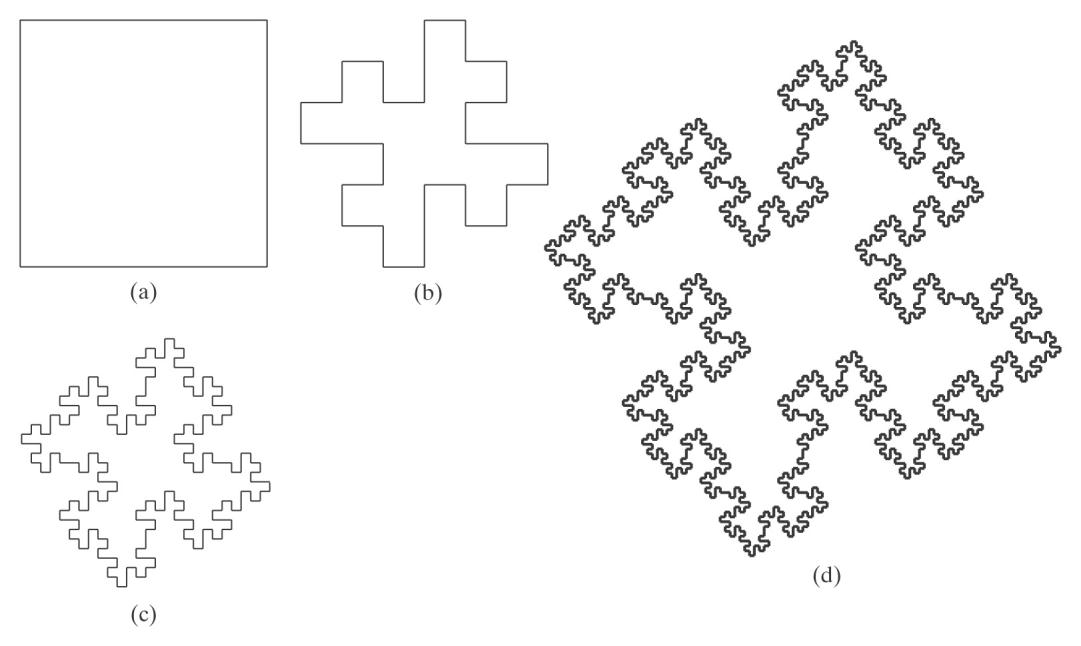
\includegraphics[scale=.4]{images/p8.png}

These figures were drawn by interpreting strings as turtle programs, just as we did in Example 24.5 and Example 24.6.  The strings were generated by an L-system $G$, defined with:

\begin{align*}
\Sigma &= \{F, +, -\}.\\
\omega &= F - F - F - F
\end{align*}

To interpret the strings as turtle programs, attach meanings to the symbols in $\Sigma$ as follows (assuming that some value for $k$ has been chosen):
\begin{itemize}
\item
$F$ means move forward, drawing a line of length $k$.
\item
$+$ means turn left $90^\circ$.
\item
$-$ means turn right $90^\circ$.
\end{itemize}

Figure (a) was drawn by the first generation string $\omega$.  Figure (b) was drawn by the second generation string, and so forth.  $R_G$ contains a single rule.  What is it?
\begin{proof}[Answer]
$F \rightarrow F + F - F - F + F + FF - F$
\end{proof}
\end{enumerate}
\end{document}
